\section{Versuchsaufbau}
%skizze zum versuchsaufbau (oder foto) einf�gen,   es muss erkl�rt werden wie das ganze funktioniert und welche speziellen einstellungen verwendet wurden (z.b. welche kn�pfe an den ger�ten f�r die messung verdreht wurden)
Der Versuchsaufbau ist in Abbildung \ref{fig:aufbau} zu sehen. Die Hauptbestandteile sind die vier Szintillatoren (PM 1-4), welche jeweils noch mit einem Photomultiplier verbunden sind.

\begin{figure}[H]
	\centering
  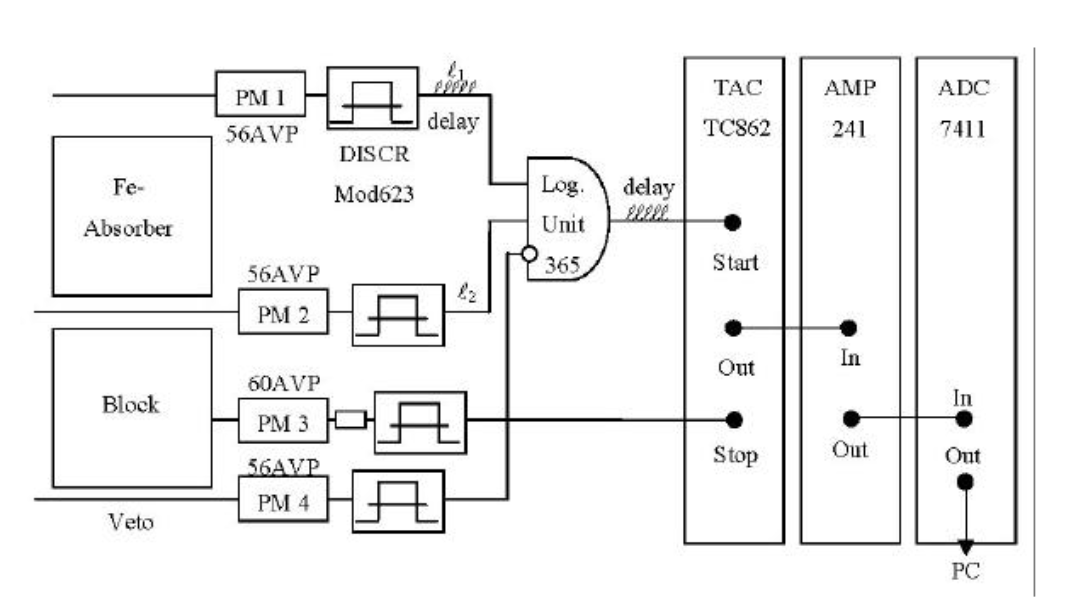
\includegraphics[scale=0.4]{unterdruekung.png}
	\caption{Schaltskizze des Versuchsaufbaus}
	\label{fig:aufbau}
\end{figure}

Der Szintillator f�r die Registrierung der Myonen ist PM3. Es handelt sich um einen 25x25x25 cm$^3$ Plastikblock-Szintillator. PM1, PM2 und PM4 sind Flach-Szintillatoren, wobei PM4 als Veto fungiert, sodass nur Ereignisse, die von PM3 noch registriert werden, jedoch nicht von PM4, gez�hlt werden. PM1, PM2 und PM4 sind �ber eine logische Einheit an den Start-Pin des TAC angeschlossen. Der TAC wird gestartet, falls PM1 und PM2 ein Ereignis registrieren und PM4 keins registriert. Wenn PM4 das Myon registriert, wird der TAC nicht gestartet, da das Myon dann nicht zerfallen ist. PM3 ist �ber den Photomuliplier an den Stop-Pin des TAC angeschlossen, sodass, nachdem die Diskriminatorschwelle auf die zweite Einstellung gestellt wurde, nur der Zerfall des Myons zu einem Signal f�hrt. Das Signal des TAC wird an einen Verst�rker (AMP) weitergeleitet, welche das Signal an einen Analog-Digital-Konverter (ADC) weitergibt. Es wurde ein Delay eingebaut, da die Szintillatoren ein unterschiedliches Baujahr haben (gr��ere Aufl�sungszeit) und sich die Kabell�nge unterscheidet. Neben dem Universit�tsgeb�ude wird ein Eisenblock als Absorber verwendet, wodurch Teilchen niedriger Energie nahezu vollst�ndig absorbiert werden und sich das Energiespektrum nach oben verschiebt. Der Vorteil des Absorbers ist, das andere Strahlung fast vollst�ndig geblockt wird.

\subsection{Diskriminator}
Ein Diskriminator wandelt ein analoges Signal in ein digitales Signal mit einer Aufl�sung von einem Bit um. Es kann eine untere Schranke eingestellt werden, ab welcher eine 0 ausgegeben wird. Zus�tzlich kann auch eine obere Schranke eingestellt werde, sodass nur bei einer Spannung zwischen den Schranken eine 1 ausgegeben wird. Es ist auch einstellbar wie lange das Signal ausgegeben wird.

\subsection{Analog-Digital-Konverter}
Ein Analog-Digital-Konverter wandelt ein analoges Spannungssignal eine in digitales Spannungssignal um. Das Aufl�sungsverm�gen wird in Bit angegeben. Je gr��er die Anzahl der Bits, desto kleinschrittiger kann das analoge Signal aufgel�st. Die Umsetzungsgeschwindigkeit gibt an, wie lange es dauert eine �nderung des analogen Signals zu digitalisieren. 

\subsection{Delay}
Da verschiedene Signale nahezu zeitgleich ankommen m�ssen, werden einzelne Signale mit einem Delay versehen. Der Delay wird meistens �ber l�ngere Kabel realisiert.

\subsection{Time-to-Amplitude-Converter(TAC)}
Ein TAC wird verwendet, um den zeitlichen Abstand zwischen zwei Ereignissen zu bestimmen. Daf�r wird beim Eintreffen eines Startsignals ein Kondensator linear aufgeladen, bis ein Stoppsignal den Strom stoppt und die Spannung an den Ausgang weitergegeben wird. Dadurch erh�lt man einen Spannungspuls der proportional zur Zeitdifferenz zwischen Start- und Stoppsignal ist. Als Besonderheit sei noch erw�hnt, dass der TAC im Jahr 1942 von Bruno Rossi zur Bestimmung der Lebensdauer von Myonen erfunden wurde.

\subsection{Multi-Channel-Analyser}
Mit einem Multi-Channel-Analyser werden Folgen von elektrischen Impulsen abh�ngig von der Gr��e einem Kanal zugeordnet und gez�hlt. Diese Daten k�nnen als Histogramm dargestellt werden, wobei jedem Kanal ein Energieintervall zugeordnet wird.

